\documentclass[conference]{IEEEtran}
\IEEEoverridecommandlockouts
\usepackage{cite}
\usepackage{amsmath,amssymb,amsfonts}
\usepackage{graphicx}
\usepackage{textcomp}
\usepackage{xcolor}
\usepackage{booktabs}
\usepackage{url}
\usepackage{hyperref}
\hypersetup{colorlinks=true,linkcolor=black,citecolor=black,urlcolor=blue}

\begin{document}

\title{Detecting Synthetic-Data Contamination in Tabular and Time-Series Training Pipelines}

\author{
\IEEEauthorblockN{Gokul Srinivasan Prabu}
\IEEEauthorblockA{Department of Artificial Intelligence and Data Science\\
Sri Krishna College of Engineering and Technology, Coimbatore, India\\
gokulsrinivasan2020@gmail.com}
}

\maketitle

\begin{abstract}
Generative models are now routinely used to enlarge scarce tabular and time-series datasets.
The resulting training mix can look statistically faithful while still degrading performance on future real observations.
This paper studies that failure mode as a data-contamination problem rather than a generator-quality contest.
We freeze a sealed real holdout that no generator is allowed to see, replace a controlled fraction of the training set with synthetic samples, and measure what happens to ordinary downstream learners.
Three generators are compared on three public tabular datasets and on Melbourne daily minimum temperatures: a Gaussian copula, independent marginal resampling, and near-duplicate jitter.
A Contamination Risk Index (CRI) packages sealed-holdout error growth, diversity collapse, and calibration drift into a bounded score.
Across 405 tabular runs, a Random Forest trained on a 70\% Gaussian-copula mix lost 6.72\% macro-F1 relative to a clean baseline, while holdout error rose by 54.3\%.
The Wine task dropped from a perfect 1.000 macro-F1 to 0.858.
On the temperature series, seasonal residual bootstrap at the same mix raised normalized MAE from 0.154 to 0.212.
Train-set Kolmogorov--Smirnov fidelity was only weakly related to sealed-holdout error (Pearson $r=0.15$).
CRI is not an independent predictor of holdout risk---half of its mass \emph{is} holdout error---but the remaining terms flag cases such as Pima diabetes, where accuracy is stable while expected calibration error rises.
The protocol is reproducible on a laptop and is intended as a gate before synthetic records enter a training warehouse.
\end{abstract}

\begin{IEEEkeywords}
synthetic data, data-centric AI, model collapse, contamination detection, time-series forecasting, tabular learning, calibration, sealed holdout
\end{IEEEkeywords}

\section{Introduction}
\IEEEPARstart{S}{ynthetic} data has moved from a privacy workaround to a default ingredient of modern learning pipelines.
Tabular generators such as CTGAN and the Synthetic Data Vault, together with time-series generators and foundation-model forecasts, are used to oversample rare classes, fill gaps, and pretrain downstream models~\cite{xu2019ctgan,zhao2021ctab,patki2016sdv,yoon2019timegan,park2018tablegan}.
The usual acceptance test is fidelity: if synthetic rows match real marginals, a practitioner treats the mix as safe.

That test is incomplete.
Recursive training on generated content can collapse diversity and shift the learner away from the true distribution, even when in-sample metrics remain strong~\cite{shumailov2024collapse,alemohammad2024mad,bertrand2024stability,dohmatob2024tails}.
Time-series foundation models add a second trap: evaluation leakage through overlapping windows, renamed series, and global shocks that are memorized rather than forecast~\cite{ansari2024chronos,meyer2025leakage}.
In both settings the scientific object is not a better generator.
It is an audit that asks whether a mixed training set will still work on data the generator never touched.

This paper makes three contributions.
First, we specify a sealed-holdout protocol in which every generator, mixer, and downstream model is forbidden from the future real split.
Second, we define a bounded Contamination Risk Index that jointly reports holdout error growth, feature-space diversity drop, and expected calibration error, and we state plainly which terms use holdout labels.
Third, we report a fully reproducible study on Breast Cancer, Wine, Pima diabetes, and daily minimum temperatures, using only public data and classical learners that a laboratory can rerun.\footnote{Code, raw runs, and this source: \url{https://github.com/Gokul7707/synthetic-data-contamination}.}

The rest of the paper is organized as follows.
Section~\ref{sec:related} reviews related work.
Section~\ref{sec:problem} states the problem.
Section~\ref{sec:method} describes the audit architecture, generators, and CRI.
Section~\ref{sec:setup} details data and implementation.
Section~\ref{sec:results} presents results.
Sections~\ref{sec:limits} and~\ref{sec:conclusion} discuss limits and conclude.

\section{Related Work}
\label{sec:related}
\paragraph{Model collapse.}
Shumailov \emph{et al.} showed that recursive training on model-generated text and images drives a degenerative feedback loop~\cite{shumailov2024collapse}.
Alemohammad \emph{et al.} described the same phenomenon as Model Autophagy Disorder (MAD): self-consuming loops amplify early artifacts until the learned distribution loses tails~\cite{alemohammad2024mad}.
Bertrand \emph{et al.} and Dohmatob \emph{et al.} analyzed iterative retraining and showed that collapse can appear as a change of scaling laws rather than a sudden crash~\cite{bertrand2024stability,dohmatob2024tails}.
Almost all of this evidence is from language or vision.
Tabular and streaming data are still thinly studied, even though they dominate operational decision systems in healthcare, energy, and finance.

\paragraph{Tabular synthesis.}
Xu \emph{et al.} introduced CTGAN for mixed-type tables~\cite{xu2019ctgan}.
Zhao \emph{et al.} proposed CTAB-GAN to handle imbalance and middle-of-the-road modes~\cite{zhao2021ctab}.
Patki, Wedge, and Veeramachaneni packaged copulas, Bayesian networks, and later deep generators in the Synthetic Data Vault~\cite{patki2016sdv}.
Related lines add differential privacy~\cite{jordon2019pategan} or fairness constraints~\cite{vanbreugel2021decaf}.
These methods are typically scored with logistic detection, pairwise correlation error, and machine-learning utility on a random test split drawn from the same pool used to fit the generator.
Utility on an in-distribution split does not answer whether a 30\% synthetic mix will still work on the next month of real arrivals.
That question is closer to classical dataset shift~\cite{quinonero2009shift} than to a generator bake-off.

\paragraph{Time-series synthesis and foundation models.}
Yoon, Jarrett, and van der Schaar proposed TimeGAN to respect temporal dynamics~\cite{yoon2019timegan}.
Chronos, TimesFM, and related foundation models now offer zero-shot forecasts from large pretraining corpora~\cite{ansari2024chronos,das2024timesfm}.
Recent audits warn that TSFM leaderboards can leak through obscure dataset overlap, resampling, and global-pattern memorization, and that token-level contamination tests from large language models do not transfer to continuous series~\cite{meyer2025leakage,li2026tsfmaudit}.
A generator that copies seasonality will look accurate until the holdout contains a regime the copy never saw.

\paragraph{Data-centric AI and valuation.}
The data-centric view argues that data quality, not architecture search, now limits deployed accuracy~\cite{ng2021datacentric,zha2023survey}.
Influence functions and Data Shapley estimate which training points help or hurt a model~\cite{koh2017influence,ghorbani2019shapley}, but they assume the training points are real.
They do not, by themselves, flag a copula clone that is distributionally close yet uninformative.
Calibration research shows that confidence can drift under shift even when accuracy moves slowly~\cite{guo2017calibration,niculescu2005predicting}.
We treat calibration drift as a contamination symptom rather than a separate reliability topic.

\paragraph{Gap.}
Prior work either (i)~proposes a new generator and reports fidelity, or (ii)~studies collapse in large generative models.
Missing is a small, sealed, modality-aware protocol that a student laboratory can run before synthetic rows are merged into a training warehouse.
This paper occupies that gap.

\section{Problem Statement}
\label{sec:problem}
Let $\mathcal{D}$ be a real dataset drawn from an unknown distribution $P_{\mathrm{real}}$.
A generator $G$, fitted only on a training slice $\mathcal{D}_{\mathrm{train}}$, produces synthetic samples $\mathcal{D}_{\mathrm{syn}}$.
A practitioner forms a mixed training set $\mathcal{D}_{\mathrm{mix}}(r)$ by replacing a fraction $r$ of $\mathcal{D}_{\mathrm{train}}$ with samples from $\mathcal{D}_{\mathrm{syn}}$, keeping the training size constant.
A downstream model $f_r$ is trained on $\mathcal{D}_{\mathrm{mix}}(r)$ and evaluated on a sealed holdout $\mathcal{D}_{\mathrm{hold}}$ that is disjoint from $\mathcal{D}_{\mathrm{train}}$ and was never shown to $G$.

The operational question is not whether $\mathcal{D}_{\mathrm{syn}}$ is indistinguishable from $\mathcal{D}_{\mathrm{train}}$ under a Kolmogorov--Smirnov (KS) test.
It is whether the risk $R(f_r,\mathcal{D}_{\mathrm{hold}})$ is materially worse than $R(f_0,\mathcal{D}_{\mathrm{hold}})$.
We want a scalar audit score $\mathrm{CRI}(r)$ that (i)~is computed without peeking at $\mathcal{D}_{\mathrm{hold}}$ during generator fitting, (ii)~rises when sealed risk rises, and (iii)~is not fooled by high-fidelity clones.

\paragraph{Problem statement.}
Given public tabular classification tasks and a real univariate series, construct generators that never see the holdout, sweep $r\in\{0,0.1,0.3,0.5,0.7\}$, and test whether sealed-holdout error, diversity, and calibration together describe contamination-induced failure better than train-set fidelity alone.

\section{Audit Protocol and Contamination Risk Index}
\label{sec:method}
Fig.~\ref{fig:arch} summarizes the pipeline.
Real records enter a sealed split.
The generator is fit only on the train slice.
Mixed sets are assembled at prescribed ratios.
Downstream models are trained on each mix.
Three parallel scores are then collected: a fidelity gap on the mixed train set, the CRI audit, and the sealed-holdout risk that stands in for future real data.

\begin{figure}[t]
\centering
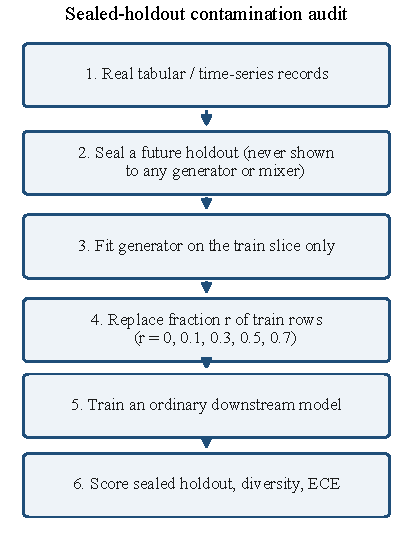
\includegraphics[width=\columnwidth]{figures/fig1_architecture.pdf}
\caption{Sealed-holdout contamination audit pipeline. The generator is never fitted on the holdout.}
\label{fig:arch}
\end{figure}

The architecture has four components.
(1)~Split control stores the holdout identity and forbids any generator call on those rows or timestamps.
(2)~The generator bank currently contains a Gaussian copula, independent marginal sampling, and near-duplicate jitter; TimeGAN or CTGAN can be dropped in without changing the rest of the pipeline.
(3)~The mixer performs sampling without replacement on real rows so that $r$ is a true replacement rate, not an append rate.
(4)~The auditor writes CRI and a pass/fail recommendation before a training job is allowed to proceed.

\subsection{Contamination Risk Index}
Let $E(r)$ be the sealed-holdout error of $f_r$.
For classification we use $E(r)=1-\mathrm{macro}$-F1.
For forecasting we use normalized MAE, $\mathrm{MAE}/\mathrm{mean}(|y_{\mathrm{hold}}|)$.
Let $\mathrm{Div}(r)$ be the mean pairwise Euclidean distance among standardized mixed-train rows (subsampled to at most 400 rows and 2000 pairs).
Let $C(r)$ be the expected calibration error (ECE) of predicted probabilities with ten equal-width bins~\cite{guo2017calibration}.
Forecasting runs set $C(r)=0$ in this study because the ridge model emits point estimates, not probabilities.

CRI is a bounded convex combination of three non-negative terms, all clipped to $[0,1]$:
\begin{equation}
\mathrm{CRI}(r)=0.5\,\Delta E(r)+0.3\,\Delta\mathrm{Div}(r)+0.2\,\Delta C(r),
\label{eq:cri}
\end{equation}
where
\begin{align}
\Delta E(r)&=\min\bigl(1,\max(0,E(r)-E(0))\bigr),\\
\Delta\mathrm{Div}(r)&=\min\bigl(1,\max(0,1-\mathrm{Div}(r)/\mathrm{Div}(0))\bigr),\\
\Delta C(r)&=\min\bigl(1,\max(0,C(r)-C(0))\bigr).
\end{align}
Relative error, $E(r)/E(0)-1$, is intentionally avoided: a perfect baseline ($E(0)=0$), which occurred on Wine for Random Forest, would explode any ratio-based index.
Weights $(0.5,0.3,0.2)$ prioritize sealed utility, then diversity, then calibration.
They are a stated design choice, not a fitted hyperparameter.

Two terms use holdout labels: $\Delta E$ is sealed error, and ECE is computed from holdout probabilities and labels.
Diversity is computed on the mixed train set only.
CRI is therefore an \emph{audit dashboard} for a laboratory that already froze a holdout, not a holdout-free predictor of future risk.
Half of its mass will track $E(r)$ by construction.
The scientific questions that remain non-circular are whether train-set fidelity ranks that risk, whether diversity or ECE move when accuracy is flat, and whether the generator family changes the curve.

\subsection{Generators and learners}
The Gaussian copula rank-transforms each train column, fits a multivariate normal on the Gaussian scale, samples, and inverts through empirical quantiles.
It preserves marginals and a linear correlation sketch~\cite{patki2016sdv}.
Independent marginals resample each column separately and destroy dependence.
Near-duplicate jitter copies real train rows and adds 5\% column-wise Gaussian noise, a high-fidelity clone that still displaces unique real records.
For classification, synthetic labels are assigned by 5-nearest neighbours in the real train set.
For the temperature series we also use seasonal residual bootstrap with period 7: a new series is grown from seasonal-naive residuals of the train slice only.

Tabular learners are $L_2$-regularized logistic regression, Random Forest (120 trees), and Histogram Gradient Boosting (max depth 6, 120 iterations).
The series model is \texttt{StandardScaler} plus Ridge regression on 14 lags.
These models are deliberately ordinary.
If contamination harms them, the audit is not an artifact of an unstable deep net.

\section{Data and Implementation}
\label{sec:setup}
\paragraph{Tabular tasks.}
We use three public classification datasets that differ in size, feature type, and difficulty (Table~\ref{tab:data}): Wisconsin Breast Cancer (569 samples, 30 numeric features, 2 classes)~\cite{wolberg1995wdbc}, UCI Wine (178 samples, 13 features, 3 classes)~\cite{aeberhard1991wine}, and the OpenML diabetes table commonly called Pima diabetes (768 samples, 8 features, 2 classes)~\cite{smith1988adap}.
Features are kept in their original units for generation so that copula quantiles remain meaningful; learners that require scaling apply a \texttt{StandardScaler} inside the training pipeline only.

\paragraph{Time series.}
We use the Melbourne daily minimum temperature series (3650 daily points), a standard public benchmark originating from the Australian Bureau of Meteorology~\cite{bommelbourne}.
A chronological 70/30 split yields a sealed future holdout; no shuffling is used.
Lag-14 windows form the supervised matrix for a ridge regressor.

\begin{table}[t]
\centering
\caption{Datasets and sealed splits.}
\label{tab:data}
\begin{tabular}{lrrrl}
\toprule
Dataset & $n$ & $d$ & Task & Split \\
\midrule
Breast Cancer & 569 & 30 & 2-class & 70/30, stratified \\
Wine & 178 & 13 & 3-class & 70/30, stratified \\
Pima diabetes & 768 & 8 & 2-class & 70/30, stratified \\
Melbourne temps & 3650 & 1 & forecast & 70/30, chronological \\
\bottomrule
\end{tabular}
\end{table}

\paragraph{Sealed protocol.}
Each tabular dataset is split 70/30 with stratification and three seeds $\{0,1,2\}$.
Generators see only the 70\% train slice.
The 30\% holdout is used solely for final scoring.
This is stricter than the common practice of fitting a generator on the full table and then sampling a test set, which silently leaks holdout structure into $\mathcal{D}_{\mathrm{syn}}$.

\paragraph{Implementation.}
All experiments were written in Python~3.12 with NumPy, pandas, SciPy, scikit-learn~1.9, and Matplotlib~\cite{pedregosa2011sklearn}.
Hardware was a standard CPU workstation; no GPU and no paid API were used.
The tabular sweep covers $3$~datasets $\times$ $3$~seeds $\times$ $3$~generators $\times$ $5$~mix ratios $\times$ $3$~models $= 405$ trained classifiers.
The series sweep covers $3$~seeds $\times$ $3$~generators $\times$ $5$~mix ratios $= 45$ ridge models.
Random seeds are fixed in the released script.
Mixed matrices keep the original training cardinality so that any change in holdout risk is attributable to composition, not to sample-size inflation.

Fidelity is reported as the mean column-wise normalized quantile gap (a KS-style statistic) between $\mathcal{D}_{\mathrm{train}}$ and $\mathcal{D}_{\mathrm{mix}}$.
A small gap means the mixed train set still looks like the real train set.
That is exactly the score a careless pipeline would trust.

\section{Results}
\label{sec:results}
\paragraph{Headline tabular result.}
Averaged over Breast Cancer, Wine, and Pima diabetes, Random Forest macro-F1 on the sealed holdout fell from 0.890 at $r=0$ to 0.830 at $r=0.7$ under Gaussian-copula replacement, a 6.72\% relative drop.
The corresponding error $1-\mathrm{macro}$-F1 rose from 0.110 to 0.170, a 54.3\% relative increase.
CRI rose from 0 to 0.036.
Logistic regression and Histogram Gradient Boosting were more sensitive: mean macro-F1 fell from 0.891 to 0.808 and from 0.890 to 0.815, respectively, at the same copula mix (Fig.~\ref{fig:heat}).

\begin{table}[t]
\centering
\caption{Random Forest under Gaussian-copula mixing (mean of 3 seeds).}
\label{tab:rf}
\begin{tabular}{lccc}
\toprule
Dataset & F1, $r=0$ & F1, $r=0.7$ & CRI at 0.7 \\
\midrule
Breast Cancer & 0.954 & 0.932 & 0.011 \\
Pima diabetes & 0.716 & 0.700 & 0.017 \\
Wine & 1.000 & 0.858 & 0.078 \\
\midrule
Mean & 0.890 & 0.830 & 0.036 \\
\bottomrule
\end{tabular}
\end{table}

Table~\ref{tab:rf} shows that contamination is task-dependent.
Wine, a small three-class problem on which the clean forest is perfect, loses 0.142 macro-F1 once 70\% of its training rows are copula clones.
Breast Cancer degrades slowly but steadily (0.954 to 0.932).
Pima diabetes is noisy at baseline; F1 is almost flat, and at $r=0.5$ it is slightly \emph{higher} (0.720 versus 0.716) while ECE rises from 0.058 to 0.088.
Accuracy-only monitoring would miss that case.
The $r=0.7$ F1 drop to 0.700 still sits inside a large seed-to-seed standard deviation (up to 0.055), so we do not treat the Pima point estimate as a sharp effect---only the calibration movement and the Wine drop are unambiguous.

\begin{figure*}[t]
\centering
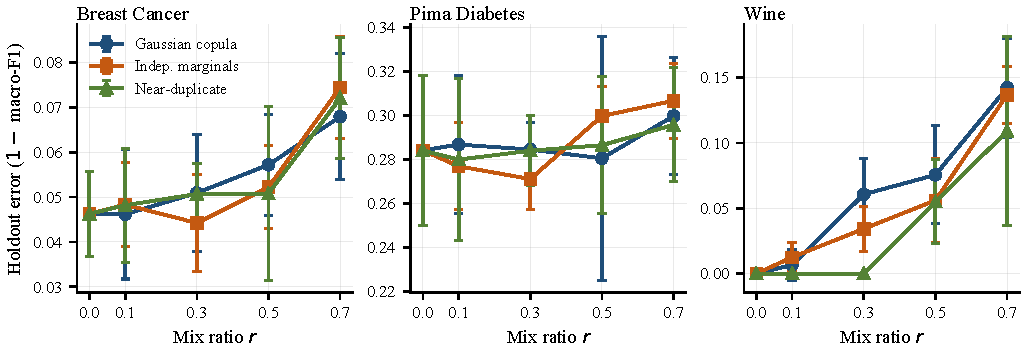
\includegraphics[width=\textwidth]{figures/fig2_tabular_error.pdf}
\caption{Sealed-holdout error of Random Forest versus synthetic mix ratio. Error bars are the standard deviation across three seeds.}
\label{fig:err}
\end{figure*}

\begin{figure}[t]
\centering
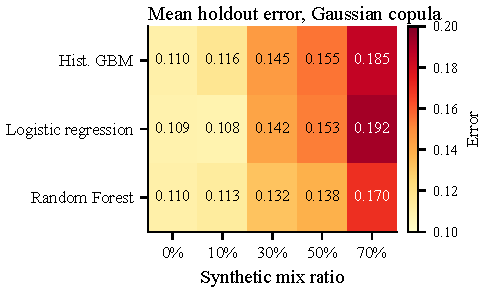
\includegraphics[width=\columnwidth]{figures/fig6_heatmap.pdf}
\caption{Mean sealed-holdout error averaged over the three tabular datasets, by learner and copula mix ratio.}
\label{fig:heat}
\end{figure}

Fig.~\ref{fig:err} and Fig.~\ref{fig:heat} make the same pattern visible: error grows with $r$ for every learner, and linear models pay a larger price than forests.
Independent marginals, which destroy feature dependence, are often as harmful as the copula.
Near-duplicates sit in between.
Averaged across tasks, no generator produced a large, consistent gain in sealed macro-F1; isolated upticks sit inside seed-to-seed variance.
Synthetic replacement is not a free lunch on these tasks.

\begin{figure}[t]
\centering
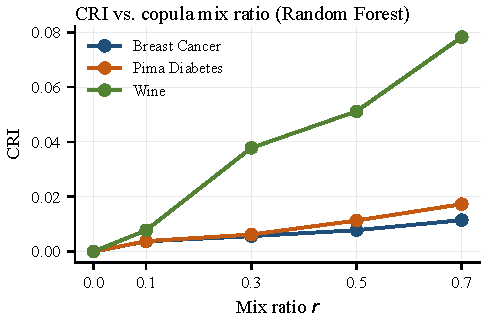
\includegraphics[width=\columnwidth]{figures/fig3_cri.pdf}
\caption{Contamination Risk Index versus copula mix ratio for Random Forest. CRI is bounded in $[0,1]$ and does not explode on the perfect Wine baseline.}
\label{fig:cri}
\end{figure}

\paragraph{Fidelity is not a sufficient statistic.}
At $r=0.7$ the near-duplicate mixer had a lower KS gap to the real train set (0.649) than the copula (0.748), as expected from cloned rows, yet Random Forest holdout error remained high (0.159 versus 0.170).
Fig.~\ref{fig:fid} plots train-mix fidelity against sealed error: the two axes are only weakly related (Pearson $r=0.15$ over 36 Random Forest conditions with $r>0$).
A pipeline that ships on KS or visual correlation heatmaps can accept a mix that later fails.

\begin{figure}[t]
\centering
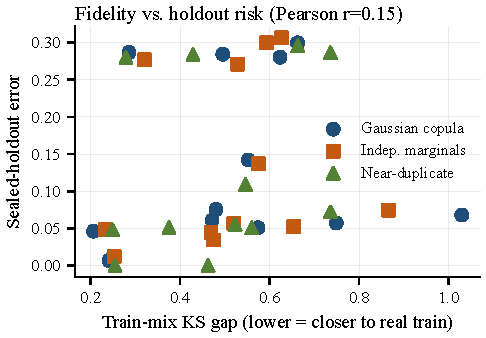
\includegraphics[width=\columnwidth]{figures/fig4_fidelity_vs_risk.pdf}
\caption{Train-set KS fidelity versus sealed-holdout error for Random Forest ($r>0$). Points that look faithful on the $x$-axis still occupy a wide range of true risk.}
\label{fig:fid}
\end{figure}

\paragraph{Time series.}
On Melbourne daily minimum temperatures, a clean ridge-on-lags model achieved normalized MAE 0.154 on the future holdout (Table~\ref{tab:ts}).
Seasonal residual bootstrap was the damaging generator: nMAE rose to 0.180, 0.193, 0.200, and 0.212 at $r=0.1,0.3,0.5,0.7$.
That is a 37.5\% relative increase at a 70\% mix.
Window copula and near-duplicate jitter barely moved nMAE (0.157 and 0.156 at $r=0.7$).
The implication is practical: a seasonal copy can poison a forecaster faster than a copula of lag windows, because it injects plausible but non-informative trajectories into the lag matrix.
Fig.~\ref{fig:ts} shows the chronological sealed split and the three generator curves.

\begin{table}[t]
\centering
\caption{Normalized MAE on the sealed future holdout (mean of 3 seeds).}
\label{tab:ts}
\begin{tabular}{lccccc}
\toprule
Generator & $r=0$ & 0.1 & 0.3 & 0.5 & 0.7 \\
\midrule
Seasonal bootstrap & 0.154 & 0.180 & 0.193 & 0.200 & 0.212 \\
Window copula & 0.154 & 0.154 & 0.155 & 0.156 & 0.157 \\
Near-duplicate & 0.154 & 0.154 & 0.155 & 0.155 & 0.156 \\
\bottomrule
\end{tabular}
\end{table}

\begin{figure*}[t]
\centering
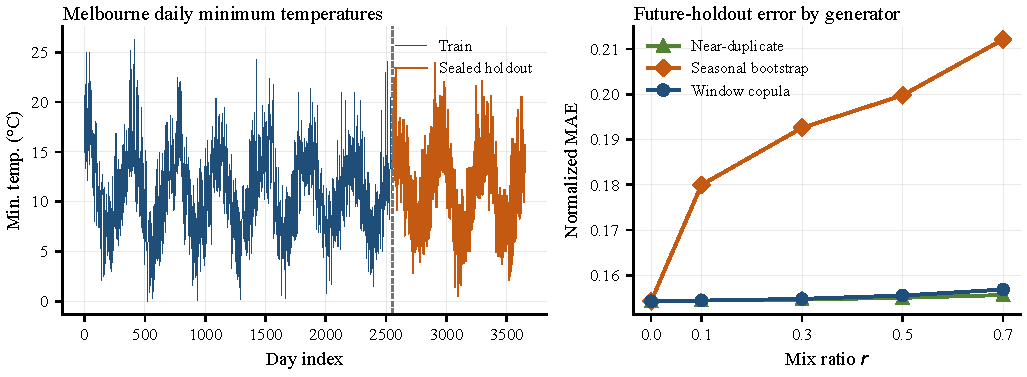
\includegraphics[width=\textwidth]{figures/fig5_timeseries.pdf}
\caption{Left: chronological train versus sealed future holdout on daily minimum temperatures. Right: normalized MAE versus mix ratio for three series generators.}
\label{fig:ts}
\end{figure*}

\paragraph{Takeaway.}
(1)~Sealed holdout error grows with synthetic replacement on ordinary learners; the effect is not reserved for large language models.
(2)~The growth is uneven across datasets, so a single accuracy threshold is unsafe.
(3)~CRI increases with $r$ and, through ECE, flags calibration-only drift on Pima at $r=0.5$.
(4)~Fidelity on $\mathcal{D}_{\mathrm{mix}}$ is a poor proxy for risk on $\mathcal{D}_{\mathrm{hold}}$.
(5)~For series, the generator family matters as much as the mix ratio: seasonal bootstrap harmed forecasts; window copula did not, at this horizon.

\section{Limitations and Future Work}
\label{sec:limits}
This is a controlled laboratory study, not a claim that every hospital or grid pipeline will lose 54\% error at a 70\% mix.
Generators are copula-class and bootstrap-class, not CTGAN, TabDDPM, or TimeGAN.
Stronger generators could be either safer (if they add true support) or more dangerous (if they copy the train set more efficiently).
The Wine baseline is perfectly separable with a forest; part of the dramatic drop is the loss of that brittle margin.
Pima's high variance across seeds means small mix effects there are not statistically sharp.
Three seeds are enough to see a trend and not enough for a formal significance test.

CRI weights were chosen, not learned, and ECE is undefined for the ridge forecaster.
Diversity uses a pairwise Euclidean proxy that can miss structured dependence collapse.
The temperature experiment is univariate.
Multivariate energy or load series, missing values, concept drift after the cutoff, and privacy attacks on the generator are out of scope.
We also do not yet test whether a CRI computed only on a labeled subset of train (without any holdout) can replace the sealed split in production; that would be a different, weaker estimator.

Four extensions follow directly.
First, drop CTGAN, TVAE, diffusion table models, and TimeGAN into the same sealed harness and ask whether deep generators change the CRI-risk curve.
Second, learn CRI weights on a meta-set of tasks so the index is a calibrated predictor of $\Delta E$ from holdout-free features only.
Third, build a leakage-free regional Indian load and monsoon holdout dated after public TSFM cutoffs, following the evaluation warnings in~\cite{meyer2025leakage,li2026tsfmaudit}.
Fourth, attach conformal prediction to the series path so $\Delta C$ is defined for forecasts, and test delayed-label streaming where synthetic backfills arrive continuously.

\section{Conclusion}
\label{sec:conclusion}
Synthetic rows can pass a train-set fidelity check and still tax the model that has to face future real data.
We framed that gap as contamination detection, not as another generator bake-off.
A sealed holdout, three simple generators, ordinary learners, and a bounded Contamination Risk Index were enough to see the effect on public tabular tasks and on a standard temperature series.
Random Forest macro-F1 fell from 0.890 to 0.830 under a 70\% copula mix; Wine fell from 1.000 to 0.858; seasonal bootstrap raised temperature nMAE from 0.154 to 0.212.
KS fidelity did not rank these failures.
The protocol is reproducible on a laptop and is intended as a gate in data-centric training pipelines, not as a finished theory of collapse.
The next step is to keep the gate and swap in stronger generators, rather than swapping the scientific question.

\section*{Acknowledgment}
The author thanks the Department of Artificial Intelligence and Data Science, Sri Krishna College of Engineering and Technology, for academic support.
All datasets used in this study are public.
Experimental figures were generated by the author from the reported runs.

\begin{thebibliography}{00}

\bibitem{xu2019ctgan}
L.~Xu, M.~Skoularidou, A.~Cuesta-Infante, and K.~Veeramachaneni, ``Modeling tabular data using conditional GAN,'' in \emph{Proc.\ NeurIPS}, 2019.

\bibitem{zhao2021ctab}
Z.~Zhao, A.~Kunar, R.~Birke, and L.~Y.~Chen, ``CTAB-GAN: Effective table data synthesizing,'' in \emph{Proc.\ ACML}, 2021.

\bibitem{patki2016sdv}
N.~Patki, R.~Wedge, and K.~Veeramachaneni, ``The Synthetic Data Vault,'' in \emph{Proc.\ IEEE DSAA}, 2016, pp.~399--410.

\bibitem{yoon2019timegan}
J.~Yoon, D.~Jarrett, and M.~van~der Schaar, ``Time-series generative adversarial networks,'' in \emph{Proc.\ NeurIPS}, 2019.

\bibitem{park2018tablegan}
N.~Park, M.~Mohammadi, K.~Gorde, S.~Jajodia, H.~Park, and Y.~Kim, ``Data synthesis based on generative adversarial networks,'' \emph{Proc.\ VLDB Endow.}, vol.~11, no.~10, pp.~1071--1083, 2018.

\bibitem{shumailov2024collapse}
I.~Shumailov, Z.~Shumaylov, Y.~Zhao, N.~Papernot, N.~Anderson, and Y.~Gal, ``AI models collapse when trained on recursively generated data,'' \emph{Nature}, vol.~631, pp.~755--759, 2024.

\bibitem{alemohammad2024mad}
S.~Alemohammad \emph{et al.}, ``Self-consuming generative models go MAD,'' in \emph{Proc.\ ICLR}, 2024.

\bibitem{bertrand2024stability}
Q.~Bertrand, J.~Bose, A.~Favero, G.~Lajoie, and P.~Vincent, ``On the stability of iterative retraining of generative models on their own data,'' in \emph{Proc.\ ICLR}, 2024.

\bibitem{dohmatob2024tails}
E.~Dohmatob, Y.~Feng, P.~Yang, F.~Charton, and J.~Kempe, ``A tale of tails: Model collapse as a change of scaling laws,'' in \emph{Proc.\ ICML}, 2024.

\bibitem{ansari2024chronos}
A.~F.~Ansari \emph{et al.}, ``Chronos: Learning the language of time series,'' \emph{Trans.\ Mach.\ Learn.\ Res.}, 2024.

\bibitem{meyer2025leakage}
M.~Meyer, S.~Kaltenpoth, K.~Zalipski, and O.~M\"uller, ``Rethinking evaluation in the era of time series foundation models: (Un)known information leakage challenges,'' arXiv:2510.13654, 2025.

\bibitem{das2024timesfm}
A.~Das, W.~Kong, R.~Sen, and Y.~Zhou, ``A decoder-only foundation model for time-series forecasting,'' in \emph{Proc.\ ICML}, 2024.

\bibitem{li2026tsfmaudit}
H.~Li, S.~Xie, L.~Shen, Z.~Li, M.~Chen, X.~Zhang, H.~Fu, J.~Sun, X.~Ren, and C.~Liu, ``TSFMAudit: Data contamination auditing in forecasting time series foundation models,'' arXiv:2605.26161, 2026.

\bibitem{ng2021datacentric}
A.~Ng, ``MLOps: From model-centric to data-centric AI,'' DeepLearning.AI, 2021.

\bibitem{zha2023survey}
D.~Zha \emph{et al.}, ``Data-centric artificial intelligence: A survey,'' \emph{ACM Comput.\ Surv.}, 2023.

\bibitem{koh2017influence}
P.~W.~Koh and P.~Liang, ``Understanding black-box predictions via influence functions,'' in \emph{Proc.\ ICML}, 2017.

\bibitem{ghorbani2019shapley}
A.~Ghorbani and J.~Zou, ``Data Shapley: Equitable valuation of data for machine learning,'' in \emph{Proc.\ ICML}, 2019.

\bibitem{guo2017calibration}
C.~Guo, G.~Pleiss, Y.~Sun, and K.~Q.~Weinberger, ``On calibration of modern neural networks,'' in \emph{Proc.\ ICML}, 2017.

\bibitem{niculescu2005predicting}
A.~Niculescu-Mizil and R.~Caruana, ``Predicting good probabilities with supervised learning,'' in \emph{Proc.\ ICML}, 2005.

\bibitem{wolberg1995wdbc}
W.~H.~Wolberg, W.~N.~Street, and O.~L.~Mangasarian, ``Breast cancer Wisconsin (diagnostic) data set,'' UCI Machine Learning Repository, 1995.

\bibitem{aeberhard1991wine}
S.~Aeberhard and M.~Forina, ``Wine data set,'' UCI Machine Learning Repository, 1991.

\bibitem{smith1988adap}
J.~W.~Smith, J.~E.~Everhart, W.~C.~Dickson, W.~C.~Knowler, and R.~S.~Johannes, ``Using the ADAP learning algorithm to forecast the onset of diabetes mellitus,'' in \emph{Proc.\ Symp.\ Comput.\ Appl.\ Med.\ Care}, 1988.

\bibitem{bommelbourne}
Australian Bureau of Meteorology, ``Daily minimum temperatures in Melbourne,'' public series used in R.~J.~Hyndman, Time Series Data Library.

\bibitem{pedregosa2011sklearn}
F.~Pedregosa \emph{et al.}, ``Scikit-learn: Machine learning in Python,'' \emph{J.\ Mach.\ Learn.\ Res.}, vol.~12, pp.~2825--2830, 2011.

\bibitem{jordon2019pategan}
J.~Jordon, J.~Yoon, and M.~van~der Schaar, ``PATE-GAN: Generating synthetic data with differential privacy guarantees,'' in \emph{Proc.\ ICLR}, 2019.

\bibitem{vanbreugel2021decaf}
B.~van~Breugel, T.~Kyono, J.~Berrevoets, and M.~van~der Schaar, ``DECAF: Generating fair synthetic data,'' in \emph{Proc.\ NeurIPS}, 2021.

\bibitem{quinonero2009shift}
J.~Qui\~{n}onero-Candela, M.~Sugiyama, A.~Schwaighofer, and N.~D.~Lawrence, \emph{Dataset Shift in Machine Learning}. Cambridge, MA: MIT Press, 2009.

\end{thebibliography}

\end{document}
